\documentclass{report}
\usepackage{amsmath}
\usepackage{txfonts}
\usepackage{amsfonts}
\usepackage{amssymb}
\usepackage{mathtools}
\usepackage{geometry}
\usepackage{color}
\usepackage{parskip}
\setlength{\parskip}{1em}
\usepackage{tikz}
\usetikzlibrary{fadings}
\usetikzlibrary{patterns}
\usetikzlibrary{shadows.blur}
\usetikzlibrary{shapes}
\usepackage{multirow}
\newcommand\parrow[3][3ex]{%
 \begin{array}[t]{@{}c@{}} #2 \\
  \left\uparrow\vcenter{\hrule height #1}\right.\kern-\nulldelimiterspace\\
  \makebox[0pt]{\small#3}
  \end{array}%
}
\newcommand\parrowlong[3][6ex]{%
 \begin{array}[t]{@{}c@{}} #2 \\
  \left\uparrow\vcenter{\hrule height #1}\right.\kern-\nulldelimiterspace\\
  \makebox[0pt]{\small#3}
  \end{array}%
}

\geometry{a4paper, margin=1in}

\begin{document}

\chapter{Partial Differential Equations in Engineering}

\section{Fundamental Lemma of ODEs}

If $\displaystyle\iiint\limits_{V} f d \tau=0$ and $\begin{aligned} 
\text { 1. } & f \text { is continuous } \\ 
\text { 2. } & V \text { is arbitrary. }\end{aligned}$

Then $f=0$ (take as fact).

Proof by contradiction:

Assume $f \neq 0$ at a point $P$. Because $f$ is continuous $f \neq 0$ in a volume $V$ surrounding $P$. (Assume $f>0$ instead of $f<0$ ).

Thus, $\displaystyle\iint\limits_{\Delta v} f d \tau>0$ (contradiction).

\begin{center}
\tikzset{every picture/.style={line width=0.75pt}}
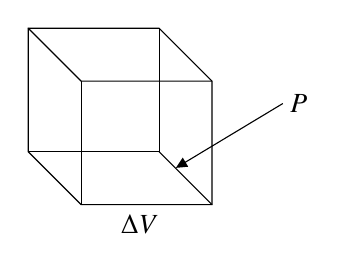
\begin{tikzpicture}[x=0.75pt,y=0.75pt,yscale=-1,xscale=1]
\draw   (248.55,123.49) -- (223.05,97.99) -- (160,97.99) -- (160,157.49) -- (185.5,182.99) -- (248.55,182.99) -- cycle ; \draw   (160,97.99) -- (185.5,123.49) -- (248.55,123.49) ; \draw   (185.5,123.49) -- (185.5,182.99) ;
\draw    (223.05,157.49) -- (160,157.49) ;
\draw    (223.05,157.49) -- (223.05,97.99) ;
\draw    (248.55,182.99) -- (223.05,157.49) ;
\draw    (282.66,134.27) -- (233.73,163.73) ;
\draw [shift={(231.16,165.27)}, rotate = 328.95] [fill={rgb, 255:red, 0; green, 0; blue, 0 }  ][line width=0.08]  [draw opacity=0] (5.36,-2.57) -- (0,0) -- (5.36,2.57) -- cycle    ;
\draw (213.5,186.39) node [anchor=north] [inner sep=0.75pt]    {$\Delta V$};
\draw (284.66,134.27) node [anchor=west] [inner sep=0.75pt]    {$P$};
\end{tikzpicture}
\end{center}

\section{Fluid Flow}

Let $S$ be a closed surface bounding volume $V$:

\begin{center}
\tikzset{every picture/.style={line width=0.75pt}} 
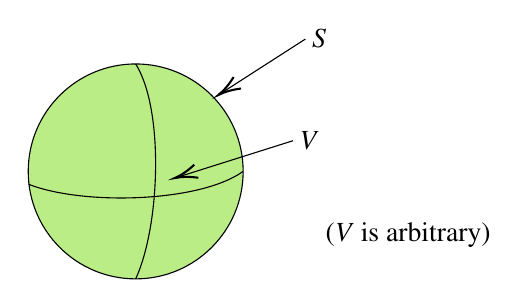
\begin{tikzpicture}[x=0.75pt,y=0.75pt,yscale=-1,xscale=1]
\draw  [fill={rgb, 255:red, 186; green, 237; blue, 134 }  ,fill opacity=1 ] (98,123.77) .. controls (98,95.18) and (121.18,72) .. (149.77,72) .. controls (178.37,72) and (201.55,95.18) .. (201.55,123.77) .. controls (201.55,152.37) and (178.37,175.55) .. (149.77,175.55) .. controls (121.18,175.55) and (98,152.37) .. (98,123.77) -- cycle ;
\draw    (149.77,72) .. controls (163.55,93.99) and (161.55,149.99) .. (149.77,175.55) ;
\draw    (201.55,123.77) .. controls (180.42,138.84) and (124.4,140.2) .. (98.19,129.99) ;
\draw    (231.55,59.99) -- (191.23,85.91) ;
\draw [shift={(189.55,86.99)}, rotate = 327.26] [color={rgb, 255:red, 0; green, 0; blue, 0 }  ][line width=0.75]    (10.93,-3.29) .. controls (6.95,-1.4) and (3.31,-0.3) .. (0,0) .. controls (3.31,0.3) and (6.95,1.4) .. (10.93,3.29)   ;
\draw    (225.55,108.99) -- (170.45,126.39) ;
\draw [shift={(168.55,126.99)}, rotate = 342.47] [color={rgb, 255:red, 0; green, 0; blue, 0 }  ][line width=0.75]    (10.93,-3.29) .. controls (6.95,-1.4) and (3.31,-0.3) .. (0,0) .. controls (3.31,0.3) and (6.95,1.4) .. (10.93,3.29)   ;
\draw (233.55,59.99) node [anchor=west] [inner sep=0.75pt]    {$S$};
\draw (227.55,108.99) node [anchor=west] [inner sep=0.75pt]    {$V$};
\draw (240,147.4) node [anchor=north west][inner sep=0.75pt]    {$( V\ \text{is arbitrary)}$};

\end{tikzpicture}
\end{center}

Rate of change of mass in $V$ is $\dfrac{d M}{d t}$

$\parrow{\dfrac{d M}{d t}}{3}= \parrow{\text{Rate of entry/(exit)}}{1} + \parrow{\text{Rate of generation/(absorption)}}{2}$

$M=\displaystyle\iiint_{V} \delta d \tau$ where $\delta$ is density.

$\therefore \dfrac{d M}{d t}=\dfrac{d}{d t} \displaystyle\iiint\limits_{V} \delta d \tau=\displaystyle\iiint\limits_{V} \dfrac{\partial \delta}{\partial t} d \tau$. (Leibniz integral rule: can swap derivative and integral).

\begin{enumerate}
    \item[(1)] $\displaystyle\oiint\limits_S\int\parrow{\vec{v}}{$\substack{\text{Velocity}\\\text{vector}}$}\cdot \parrowlong{\vec{n}}{$\substack{\text{unit normal}\\
    \text{vector}}$}dS=-\oiint\limits_S\delta\vec{v}\cdot \vec{n}\parrow{dS}{Surface element}$\quad (\text{hand wavey - but $m'=\delta$}).

    \begin{center}
\tikzset{every picture/.style={line width=0.75pt}} 
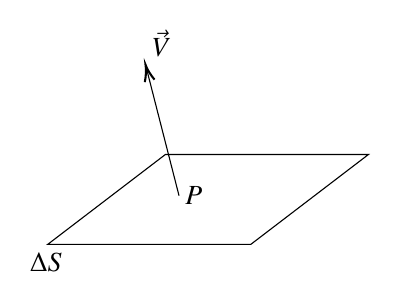
\begin{tikzpicture}[x=0.55pt,y=0.55pt,yscale=-1,xscale=1]
\draw   (158.55,138.99) -- (291.96,138.99) -- (214.73,197.99) -- (81.31,197.99) -- cycle ;
\draw    (167.55,165.99) -- (146.04,81.93) ;
\draw [shift={(145.55,79.99)}, rotate = 75.65] [color={rgb, 255:red, 0; green, 0; blue, 0 }  ][line width=0.75]    (10.93,-3.29) .. controls (6.95,-1.4) and (3.31,-0.3) .. (0,0) .. controls (3.31,0.3) and (6.95,1.4) .. (10.93,3.29)   ;
\draw (169.55,165.99) node [anchor=west] [inner sep=0.75pt]    {$P$};
\draw (147.55,76.59) node [anchor=south west] [inner sep=0.75pt]    {$\vec{V}$};
\draw (81.31,201.39) node [anchor=north] [inner sep=0.75pt]    {$\Delta S$};
\end{tikzpicture}
    \end{center}

    \item[(2)] Let $Q(\vec{r}, t)$ be the rate at which fluid is generated/(absorbed). t is time, $\vec{r}$ is the position vector. Unit of $Q$ is (ie.) $g / c c / s$.

    $\therefore$ Net generation/(absorption) is.

    \item[(2)] $=\iiint_{V} Q(\vec{r}, t) d \tau$. 
\end{enumerate}

dell operator $\left(\frac{\partial F_{1}}{\partial x}+\frac{\partial F_{2}}{\partial y}+\frac{\partial F_{3}}{\partial z}\right)$.\\


By the Divergence Theorem: $\displaystyle\oiint\limits_{S} \vec{F} \cdot d \vec{S}=\iiint\limits_{V} \vec{\nabla} \cdot \vec{F} d v$

$\therefore$ (1) $=\displaystyle-\iiint\limits_{\tau} \vec{\nabla} \cdot \delta \vec{v} d \tau \quad$ integration in (1) and (2) done over same volume. (arbitrary)

$$
\displaystyle\iiint_{\tau}\left[\dfrac{\partial \delta}{\partial t}+\vec{\nabla} \cdot(\delta \vec{v})-Q\right] \delta \tau=\dfrac{d M}{d t}=0
$$

$\therefore$ By Fundamental Lemma: $\dfrac{\partial \delta}{\partial t}+\vec{\nabla} \cdot(\delta \vec{v})-Q=0$ ``Law of Conservation of Mass''

This can be further simplified if special conditions are met.

If incompressible ( $\delta$ constant): $0+\delta \vec{\nabla} \cdot \vec{v}=Q. \quad \therefore \vec{\nabla} \cdot \vec{v}=Q / \delta$

If also irrotational (no swirling $\rightarrow \vec{\nabla} \times \vec{v}=\overrightarrow{0}$ )

$\therefore \vec{\nabla}=\vec{\nabla} \psi\left(\dfrac{\partial \psi}{\partial x}, \dfrac{\partial \psi}{\partial y}, \dfrac{\partial \psi}{\partial z}\right).$ \quad  (curl =0)

* See the water flowing down a hill analogy. $\psi$= ``scalar potential''.


$\therefore \nabla^{2} \psi=Q / \delta$. \}``Poisson's Equation''.

If also $Q=0$ (no fluid generated/consumed).

$$
\left.\therefore \nabla^{2} \psi=0\right\} \text { ``Laplace's Equation'' (with } \vec{v}=\vec{\nabla} \psi)
$$

\section{Diffusion of Heat} 

$\psi(\vec{r}, t)$ is temperature at direction vector $\vec{r}$ at time $t$.

Let $S$ be a closed surface bounding volume $V$:

\begin{center}
\tikzset{every picture/.style={line width=0.75pt}} 
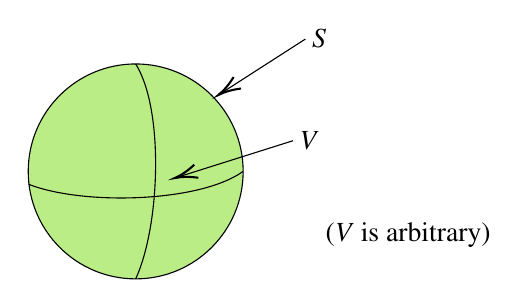
\begin{tikzpicture}[x=0.75pt,y=0.75pt,yscale=-1,xscale=1]
\draw  [fill={rgb, 255:red, 186; green, 237; blue, 134 }  ,fill opacity=1 ] (98,123.77) .. controls (98,95.18) and (121.18,72) .. (149.77,72) .. controls (178.37,72) and (201.55,95.18) .. (201.55,123.77) .. controls (201.55,152.37) and (178.37,175.55) .. (149.77,175.55) .. controls (121.18,175.55) and (98,152.37) .. (98,123.77) -- cycle ;
\draw    (149.77,72) .. controls (163.55,93.99) and (161.55,149.99) .. (149.77,175.55) ;
\draw    (201.55,123.77) .. controls (180.42,138.84) and (124.4,140.2) .. (98.19,129.99) ;
\draw    (231.55,59.99) -- (191.23,85.91) ;
\draw [shift={(189.55,86.99)}, rotate = 327.26] [color={rgb, 255:red, 0; green, 0; blue, 0 }  ][line width=0.75]    (10.93,-3.29) .. controls (6.95,-1.4) and (3.31,-0.3) .. (0,0) .. controls (3.31,0.3) and (6.95,1.4) .. (10.93,3.29)   ;
\draw    (225.55,108.99) -- (170.45,126.39) ;
\draw [shift={(168.55,126.99)}, rotate = 342.47] [color={rgb, 255:red, 0; green, 0; blue, 0 }  ][line width=0.75]    (10.93,-3.29) .. controls (6.95,-1.4) and (3.31,-0.3) .. (0,0) .. controls (3.31,0.3) and (6.95,1.4) .. (10.93,3.29)   ;
\draw (233.55,59.99) node [anchor=west] [inner sep=0.75pt]    {$S$};
\draw (227.55,108.99) node [anchor=west] [inner sep=0.75pt]    {$V$};
\draw (240,147.4) node [anchor=north west][inner sep=0.75pt]    {$( V\ \text{is arbitrary)}$};

\end{tikzpicture}
\end{center}


Rate of change of heat = Rate of entry/(exit) + Rate of generation/(absorption.).

* Like for fluid flow.

$$
(3)=(1)+(2)
$$

Solving for (3). 

The amount of heat in a small mass element $(\Delta m=\delta \Delta \tau)$ is: $\approx[c \psi(\vec{r}, t) \delta]_{p} \Delta \tau$

\begin{center}
\tikzset{every picture/.style={line width=0.75pt}} 
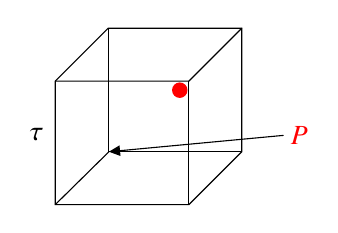
\begin{tikzpicture}[x=0.75pt,y=0.75pt,yscale=-1,xscale=1]
\draw   (90.11,143.49) -- (115.61,117.99) -- (180,117.99) -- (180,177.49) -- (154.5,202.99) -- (90.11,202.99) -- cycle ; \draw   (180,117.99) -- (154.5,143.49) -- (90.11,143.49) ; \draw   (154.5,143.49) -- (154.5,202.99) ;
\draw    (115.99,177.49) -- (180,177.49) ;
\draw    (115.99,177.49) -- (115.99,117.99) ;
\draw    (90.11,202.99) -- (115.99,177.49) ;
\draw    (200.11,169.61) -- (118.98,177.21) ;
\draw [shift={(115.99,177.49)}, rotate = 354.65] [fill={rgb, 255:red, 0; green, 0; blue, 0 }  ][line width=0.08]  [draw opacity=0] (5.36,-2.57) -- (0,0) -- (5.36,2.57) -- cycle    ;
\draw  [draw opacity=0][fill={rgb, 255:red, 255; green, 0; blue, 0 }  ,fill opacity=1 ] (146.39,147.83) .. controls (146.39,145.77) and (148.06,144.11) .. (150.11,144.11) .. controls (152.17,144.11) and (153.84,145.77) .. (153.84,147.83) .. controls (153.84,149.89) and (152.17,151.56) .. (150.11,151.56) .. controls (148.06,151.56) and (146.39,149.89) .. (146.39,147.83) -- cycle ;
\draw (81,164.89) node [anchor=north] [inner sep=0.75pt]    {$\tau $};
\draw (202.11,169.61) node [anchor=west] [inner sep=0.75pt]  [color={rgb, 255:red, 255; green, 0; blue, 0 }  ,opacity=1 ]  {$P$};
\end{tikzpicture}
\end{center}

$\therefore H=\iiint\limits_{\tau} c \delta \psi d \tau$ differentiate both sides and apply Leibniz' Rule.


\begin{equation*}
\therefore \dfrac{d H}{d t}=\iiint\limits_{\tau} \dfrac{\partial}{\partial t}[c \delta \psi] d \tau \tag{3}
\end{equation*}


Solving for (1).

Heat flows from hot to cold (entropy).

\begin{center}
\tikzset{every picture/.style={line width=0.75pt}}
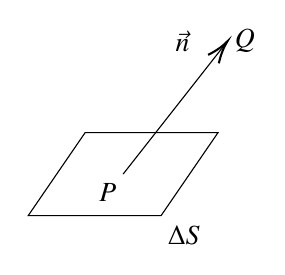
\begin{tikzpicture}[x=0.75pt,y=0.75pt,yscale=-1,xscale=1]
\draw   (105.98,127) -- (170,127) -- (142.56,167) -- (78.55,167) -- cycle ;
\draw    (124.27,147) -- (173.31,84.56) ;
\draw [shift={(174.55,82.99)}, rotate = 128.15] [color={rgb, 255:red, 0; green, 0; blue, 0 }  ][line width=0.75]    (10.93,-3.29) .. controls (6.95,-1.4) and (3.31,-0.3) .. (0,0) .. controls (3.31,0.3) and (6.95,1.4) .. (10.93,3.29)   ;
\draw (157.55,82.99) node [anchor=east] [inner sep=0.75pt]    {$\vec{n}$};
\draw (176.55,82.99) node [anchor=west] [inner sep=0.75pt]    {$Q$};
\draw (122.27,150.4) node [anchor=north east] [inner sep=0.75pt]    {$P$};
\draw (144.56,170.4) node [anchor=north west][inner sep=0.75pt]    {$\Delta S$};
\end{tikzpicture}
\end{center}

I.e. heat will leave the surface if $\psi(P)>\psi(Q)$ (along normal)

Rate at which heat leaves $\Delta S$ is: 

$$
\approx-\left[K \dfrac{\partial \psi}{\partial n}\right]_{p} \Delta S
$$

($K=$ conductivity).

This means that net heat exit if $\dfrac{\partial \psi}{\partial n}<0\ (\psi(P)>\psi(Q))$. Net rate of heat entry is $\oiint k \dfrac{\partial \psi}{\partial n} d s=$ (1)

If (1) is positive, net heat in.

Solving for (2):

Simply, if $Q(\vec{r}, t)$ is rate of heat generation/(absorption) as cal/c.c./sec, then:

Net heat gen./(abs.) is

$$
(2)=\iiint\limits_{V} Q(\vec{r}, t) d \tau
$$

Before combining, use Divergence Theorem on (1)

$\oiint k \dfrac{\partial \psi}{\partial n} d S=\oiint  K \nabla \vec{\psi} \cdot \vec{n} d S=\iiint\limits_{V} \vec{\nabla}(K \nabla \vec{\psi}) d \tau \quad$ Triple Integral, can combine.


\begin{equation*}
\iiint\limits_{\tau} \dfrac{\partial}{\partial t}[c \delta \psi] d \tau=\iiint\limits_{V} \vec{\nabla}(K \vec{\nabla} \psi) d \tau+\iiint\limits_{V} Q(\vec{r}, t) d \tau
\end{equation*}


Move everything to same side:

$$
\underbrace{\iiint_{\tau}}_{\text {Arbitrary}} \underbrace{\left[\dfrac{\partial}{\partial t}[c \delta \psi]-\vec{\nabla}(K \vec{\nabla} \psi)-Q(\vec{r}, t)\right]}_{\text{Assume continuous}} d \tau=0.
$$

By Fundamental Lemma: $\dfrac{\partial}{\partial t}[c \delta \psi]-\vec{\nabla}(K \vec{\nabla} \psi)-Q(\vec{r}, t)=0$.

If $c, K, \delta$ all constant: $c \delta \dfrac{\partial \psi}{\partial t}-K \nabla^{2} \psi-Q(\vec{r}, t)=0$

$\left.\therefore \dfrac{1}{\alpha^{2}} \dfrac{\partial \psi}{\partial t}-\nabla^{2} \psi=\dfrac{Q}{K}\right\}$ ``\text{Fourier Diffusion Equation}'' ($\alpha^{2}=\dfrac{K}{\delta c}$, ``\text{diffusivity}'')

If $Q=0: \dfrac{1}{\alpha^{2}} \dfrac{\partial \psi}{\partial t}-\nabla^{2} \psi=0=\left[\dfrac{1}{\alpha^{2}} \dfrac{\partial}{\partial t}-\nabla^{2}\right] \psi=0$ For a Steady State, Temperature is time  invariant. $\left(\frac{\partial}{\partial t}=0\right)$.

If steady state:

$\left.\nabla^{2} \psi=-Q / k\right\}$ ``Poisson's Equation''

If also $Q=0$:

$\left.\nabla^{2} \psi=0\right\}$ ``Laplace's Equation''

\section{Vibrating String}

\begin{center}
\tikzset{every picture/.style={line width=0.75pt}} 
\begin{tikzpicture}[x=0.75pt,y=0.75pt,yscale=-1,xscale=1]
\draw    (104.55,139.99) -- (376.55,139.99) ;
\draw    (105.55,164.99) -- (105.55,95.99) ;
\draw    (104.55,139.99) .. controls (122.55,116.99) and (129.55,102.99) .. (145.55,106.99) .. controls (161.55,110.99) and (171.27,163.35) .. (199.55,167.99) .. controls (227.82,172.63) and (240.34,113.36) .. (259.55,107.99) .. controls (278.75,102.62) and (284.45,156.69) .. (304.55,159.99) .. controls (324.64,163.29) and (341.22,123.73) .. (347.55,118.99) ;
\draw (103.55,92.59) node [anchor=south east] [inner sep=0.75pt]    {$\psi $};
\draw (376.55,143.39) node [anchor=north] [inner sep=0.75pt]    {$x=l$};
\draw (105.55,168.39) node [anchor=north] [inner sep=0.75pt]    {$x=0$};
\end{tikzpicture}
\end{center}

Displacement $\psi$ is a function of time and position

$a^2\dfrac{\partial^2\psi}{\partial x^2}-\dfrac{\partial^2}{\partial t^2}=-F$

$F=\dfrac{\text{Force}}{\text{Mass}},\quad a=\sqrt{\dfrac{T}{\delta}}$

$T$ = Tension\\
$\delta$ = Linear Density\\

General solution to the PDE is: $\psi=\underbrace{F(x-a t)}_{\text{moving right}}+\underbrace{G(x+a t)}_{\text{moving left}}$ ``with speed $a$''

* Derivation and solution in coursepack.

For an ``infinite'' string:

$\psi(x, t)=\dfrac{f(x-a t)+f(x+a t)}{2}+\dfrac{1}{2 a} \displaystyle\int_{x-a t}^{x+a t} g(\xi) d \xi,$ I.C. $\begin{array}{l}
     \psi(x,0)=f(x)  \\
     \psi(t,0)=g(x)
\end{array}$

e.g $f(x)=\sin(x)\quad g(x)=xe^{-x^2}$

$\begin{aligned}
    & \psi(x, t)=\dfrac{\sin (x-a t)+\sin (x+a t)}{2}+\dfrac{1}{2 a} \displaystyle\int_{x-a t}^{x+a t} \xi x e^{-\xi^{2}} d \xi\\
    & =\sin (x) \cos (a t)-\dfrac{1}{4 a}\left[e^{-\xi^{2}}\right]_{x-a t}^{x+a t}
\end{aligned}$


\section{Vibrating Membrane}


$F=m a$ and external forces $\Rightarrow \oiint$

Tension forces $\Rightarrow \oint$

For static deflections: $\dfrac{\partial^{2} \psi}{\partial t^{2}}=0$

strings (1D): $a \dfrac{\partial^{2} \psi}{\partial x^{2}}=-F$

membranes (2D): $\left.\nabla^{2} \psi=-F / a^{2}\right\}$ ``Poisson's Equation''

\section{Three Fundamental Equations}
There are three significant PDEs that govern many engineering systems
\begin{enumerate}
  \item Poisson's Equation

  $\left.\nabla^{2} \psi=-F\right\}$ if 0, Laplace's (special case of Poisson's).
  
  \item Diffusion Equation

  $\nabla^{2} \psi-\dfrac{1}{\alpha^{2}} \dfrac{\partial \psi}{\partial t}=-F$

  \item Wave Equation

  $a^{2} \nabla^{2} \psi-\dfrac{\partial^{2} \psi}{\partial t^{2}}=-F$
\end{enumerate}


Many (but not all) DE are governed by one of there 3 equations.

\section{Solving PDEs}

For the homogeneous Wave equation: 

$a^{2} \dfrac{\partial^{2} \psi}{\partial x^{2}}-\dfrac{\partial^{2} \psi}{\partial t^{2}}=0, \quad$ we have a general solution.

$$\psi(x,t)=F(x-at)+G(x+at)$$

Eg. $\begin{array}[t]{lll}
     f(z) & = & z^{2}=(x+i y)^{2}\\
     & = & x^{2}+2 i x y-y^{2}\\
     & = & x^{2}-y^{2}+i(2 x y)=u(x, y)+i v(x, y)
\end{array}$

$\left.\begin{array}{l}
     u(x, y)=x^{2}-y^{2}\\
     v(x, y)=2 x y     
\end{array}\right\}\quad \begin{array}{l}
     \nabla^{2} u=2-2=0\\
     \nabla^{2} V=0 
\end{array}$

The two functions generates two harmonics. This is common. For a well-posed problem, we need a unique solution

\textbf{1. Dirichlet B.C.}

Value of $u$ is constant with time on boundary.

\begin{center}
\tikzset{every picture/.style={line width=0.75pt}}
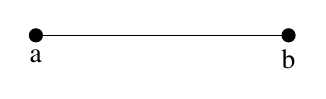
\begin{tikzpicture}[x=0.55pt,y=0.55pt,yscale=-1,xscale=1]
\draw  [draw opacity=0][fill={rgb, 255:red, 0; green, 0; blue, 0 }  ,fill opacity=1 ] (95.34,103) .. controls (95.34,100.43) and (97.43,98.34) .. (100,98.34) .. controls (102.57,98.34) and (104.66,100.43) .. (104.66,103) .. controls (104.66,105.57) and (102.57,107.66) .. (100,107.66) .. controls (97.43,107.66) and (95.34,105.57) .. (95.34,103) -- cycle ;
\draw  [draw opacity=0][fill={rgb, 255:red, 0; green, 0; blue, 0 }  ,fill opacity=1 ] (261.34,103) .. controls (261.34,100.43) and (263.43,98.34) .. (266,98.34) .. controls (268.58,98.34) and (270.66,100.43) .. (270.66,103) .. controls (270.66,105.57) and (268.58,107.66) .. (266,107.66) .. controls (263.43,107.66) and (261.34,105.57) .. (261.34,103) -- cycle ;
\draw    (100,103) -- (266,103) ;
\draw (100,110.66) node [anchor=north] [inner sep=0.75pt]   [align=left] {a};
\draw (266,110.66) node [anchor=north] [inner sep=0.75pt]   [align=left] {b};
\end{tikzpicture}
\end{center}

$$
\left\{\begin{array}{l}
u(a, t)=0 \\
u(b, t)=0
\end{array}\right. \quad \forall t.
$$

\textbf{2. Neumann B.C.}

Spatial derivative of $u$ is constant with time on boundary.

\begin{center}
\tikzset{every picture/.style={line width=0.75pt}} 
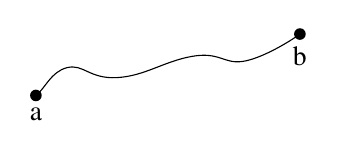
\begin{tikzpicture}[x=0.45pt,y=0.45pt,yscale=-1,xscale=1]
\draw    (133,166) .. controls (140.65,160.26) and (144.91,147.01) .. (158,143.68) .. controls (171.09,140.35) and (175.85,152.84) .. (198,151.68) .. controls (220.16,150.51) and (235.57,138.74) .. (258,134.68) .. controls (280.44,130.61) and (283.83,140.87) .. (299,138.68) .. controls (314.18,136.48) and (337.2,122.53) .. (345,116.68) ;
\draw  [draw opacity=0][fill={rgb, 255:red, 0; green, 0; blue, 0 }  ,fill opacity=1 ] (128.34,166) .. controls (128.34,163.43) and (130.43,161.34) .. (133,161.34) .. controls (135.57,161.34) and (137.66,163.43) .. (137.66,166) .. controls (137.66,168.57) and (135.57,170.66) .. (133,170.66) .. controls (130.43,170.66) and (128.34,168.57) .. (128.34,166) -- cycle ;
\draw  [draw opacity=0][fill={rgb, 255:red, 0; green, 0; blue, 0 }  ,fill opacity=1 ] (340.34,116.68) .. controls (340.34,114.1) and (342.43,112.02) .. (345,112.02) .. controls (347.58,112.02) and (349.66,114.1) .. (349.66,116.68) .. controls (349.66,119.25) and (347.58,121.34) .. (345,121.34) .. controls (342.43,121.34) and (340.34,119.25) .. (340.34,116.68) -- cycle ;
\draw (133,173.66) node [anchor=north] [inner sep=0.75pt]   [align=left] {a};
\draw (345,124.34) node [anchor=north] [inner sep=0.75pt]   [align=left] {b};
\end{tikzpicture}
\end{center}

$$
\left\{\begin{array}{l}
u_{x}(a, t)=0 \\
u_{x}(b, t)=0
\end{array} \quad \forall t\right.
$$

\textbf{3. Robin B.C.}

A linear combination of Dirichelet and Neumann.

$$
A u(a, t)+B u_{x}(a, t)=c, \quad \forall t
$$

\section{Uniqueness Theorems}

``For Poisson's Equation (or Laplace's), the solution of a Dirichlet problem is unique, and Neumann problem is unique to an additive constant."


\textbf{Proof:} Let $\psi_{1}$ and $\psi_{2}$ be two solutions to the same problem, i.e:

$\nabla^{2} \psi_{1}=-F$ and $\left.\nabla^{2} \psi_{2}=-F\right\}$\qquad Goal: Prove $\psi_{1}=\psi_{2}$ for Dirichlet and $\psi_{1}-\psi_{2}=c$ for Neumann

either $\left[\Psi_{1}\right]_{s}=\left[\psi_{2}\right]_{s}$ (Dirichlet) 

or $\left[\dfrac{\partial \psi_{1}}{\partial n}\right]_{s}=\left[\dfrac{\partial \psi_{2}}{\partial n}\right]_{s}$ (Neumann)

Let $U=\psi_{1}-\psi_{2}$, then $\nabla^{2} U=\nabla^{2} \psi_{1}-\nabla^{2} \psi_{2}=-F-(-F)=0$ on $\tau.$

Either $[u]_{s}=0$ (Dirichlet) 
or. 

$\left[\dfrac{\partial u}{\partial n}\right]_{S}=0$ (Neumann)

for this to hold true.

Consider $\oiint\limits_{s} u \dfrac{\partial u}{\partial n} d S=0$, this is equal to $\oiint\limits_{s} U \overrightarrow{\nabla U} \cdot \vec{n} d S \quad$ (Def. of nabla operator).

Applying Divergence Theorem:

$0=\iiint\limits_{\tau} \vec{\nabla} \cdot[u \overrightarrow{\nabla u}] d \tau \quad$ Apply vector identity (Product Rule) from Tutorial 1 .


$0=\iiint\limits_{\tau} \underbrace{\overrightarrow{\nabla u} \cdot \overrightarrow{\nabla u}}_{\|\overrightarrow{\nabla u}\|^{2}} d \tau+\iiint\limits_{\tau} u \underbrace{\nabla^{2} u}_{=0} d \tau
$

However, we may not automatically conclude $\|\overrightarrow{\nabla u}\|^{2}=0$ by the Fundamental Lemma since $\tau$ is not arbitrary.

Instead, we use the limit of a sum argument for integrals because $\|\vec{\nabla}\|^{2} \geqslant 0$.

And $\iiint\limits_{\tau} \underbrace{\|\vec{\nabla u}\|^{2}}_{\geq 0} d \tau=0 \quad$ 

$\therefore\|\overrightarrow{\nabla u}\|^2=0$ in $\tau$

$\therefore\overrightarrow{\nabla u}=0\quad\Rightarrow\quad u=\psi_1-\psi_2=c$ in $\tau$.

This proves the Neumann part.

For Dirichlet, we have $[u]_{s}=0$ and $[u]_{\tau}=c$

Since $\tau$ can be infinitesimally close to $s$, we can't continuously go from 0 on $S$ to $c$ on $\tau$, if $c \neq 0$ $\therefore c=0 \Rightarrow \psi_{1}=\psi_{2}$, which proves Dirichelet.

Note on arbitrary domains:

Consider $\displaystyle\int_{\tau} x d x$. This is clearly not always zero. However, if domain $\tau=x \in[-1,1]$, then $\displaystyle\int_{-1}^{1} x d x=0$. This doesn't mean $x$ is zero, since the domain is not arbitrary. This is the definition of ``arbitrary $\tau$'' in the Fundamental Lemma. It can only be applied if the domain is arbitrary (and thus integral = 0 regardless of bounds).

``For Poisson's Equation (or Laplace's), the solution of a Robin problem is unique.

\textbf{Proof:} Let $\psi_{1}$ and $\psi_{2}$ be two solutions to the same problem, i.e:

$\nabla^{2} \psi_{1}=-F$ and $\nabla^{2} \psi_{2}=-F$ in $\tau$.

$\dfrac{\partial \psi_{1}}{\partial n}+h \psi_{1}=\dfrac{\partial \psi_{2}}{\partial n}+h \psi_{2}$ on $s$. the boundary of $\tau$, with $h$ positive.

Let $u=\psi_{1}-\psi_{2}$, then $\nabla^{2} u=0$ in $\tau$.

$$
\dfrac{\partial}{\partial n}\left(\psi_{1}-\psi_{2}\right)+h\left(\psi_{1}-\psi_{2}\right)=0 \text { or } \frac{\partial u}{\partial n}+h u=0 \text { on } s .
$$

Now, $\oiint\limits_{s} u \dfrac{\partial u}{\partial n} d S=-\oiint\limits_{s} h u^{2} d S \quad\left(b c \cdot \frac{\partial u}{\partial n}=-h u\right)$

$$
=\oiint_{s} u \overrightarrow{\nabla u} \cdot \stackrel{\rightharpoonup}{n} d S \underset{\text { Theorem }}{\substack{\text { Divergence }}} \iiint_{\tau} \vec{\nabla} \cdot(u \overrightarrow{\nabla u}) d \tau
$$

Only way for L.H.S. = R.H.S. is if both are $0$.

$\iiint\limits_{\tau}\|\overrightarrow{\nabla u}\|^{2} d \tau=0 \Rightarrow u=$ constant in $\tau$.

$$
\oiint_{s} \underbrace{h u^{2}}_{\geqslant 0} d s=0 \Rightarrow u=0 \text { on } s.
$$

Hence by continuity, $u=\psi_{1}-\psi_{2}=0$, thus $\psi_{1}=\psi_{2}$.

Theorem 3: For the diffusion equation, solutions of Dirichlet and Neumann problems are unique if $\psi(\vec{r}, 0)$ is specified.

Theorem 4: For the wave equation, solutions of Dirichlet and Neumann problems are unique if $\psi(\vec{r}, 0)$ and $\psi_{+}(\vec{r}, 0)$ is specified.

(Proofs not needed).

\end{document}
